\documentclass[a4paper,11pt,oneside,showtrims]{alpenthesis}
\usepackage{lipsum}
\hextrue
\paperfalse

%% ================================================================= SET TITLE %
\title{My Thesis}
\author{Raphael Frey \\[1ex]\href{https://github.com/alpenwasser/}
                                 {\nolinkurl{https://github.com/alpenwasser/}}}

\chapterstyle{alpenthesis}
%% ============================================================== END PREAMBLE %
\begin{document}
%% ============================================================= BEGIN CONTENT %
\begin{titlingpage}
    \fullhexpage{dv-7}{dv-5}
    \tikzset{external/export next=false}%
    \begin{tikzpicture}[remember picture,overlay]
        \node[anchor=north east,yshift=-5mm,xshift=-10mm]
            at (current page.north east)
            {
\includegraphics[height=10mm]{logo-top.pdf}};
    \end{tikzpicture}
    \tikzset{external/export next=false}%
    \begin{tikzpicture}[remember picture,overlay]
        \node[anchor=south east,yshift=+5mm,xshift=-10mm]
            at (current page.south east)
            {
\includegraphics[height=16mm]{logo-bottom.pdf}};
    \end{tikzpicture}
    \flushright\sffamily

    \vspace{3ex}
    \Huge\bfseries{A Mostly Appropriate Title}\\[1ex]
    \Large\mdseries{Thesis}\\[3ex]

    \normalsize\mdseries

    alpenwasser\\
    team partner\\[3ex]

    Supervisor\\
    Expert\\

    \vfill

    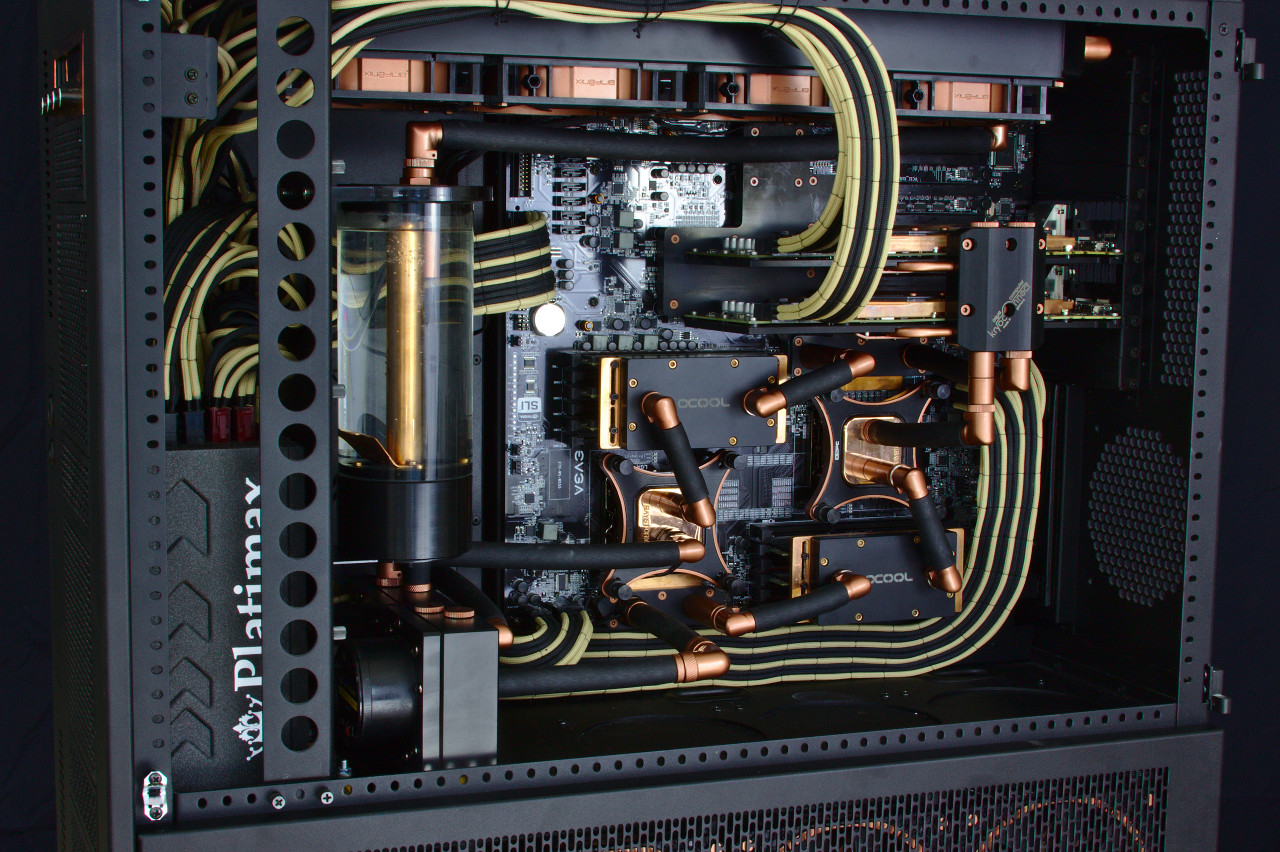
\includegraphics[width=120mm]{titlepic.jpg}

    \vfill

    \today\\
    Version 1.0.0
\end{titlingpage}
\frontmatter
\tableofcontents*

\mainmatter
\chapter{Text}
\lipsum[1]

\sffamily\lipsum[2]

\bfseries\lipsum[3]

\mdseries\ttfamily\lipsum[4]

\bfseries\ttfamily\lipsum[5]

\normalfont\scshape\lipsum[6]

\slshape\lipsum[7]

\scshape\lipsum[8]

\scslshape\lipsum[9]

\normalfont

\chapter{Tables}
\begin{table}
    \centering
    \caption{tabular inside float}
    \label{tab:float}
    \begin{tabular}{lll}
        \toprule
        \scshape Header 1 & \scshape Header 2 & \scshape Header 3 \\
        \midrule
        Content           & Content           & Content           \\
        Content           & Content           & Content           \\
        Content           & Content           & Content           \\
        Content           & Content           & Content           \\
        \bottomrule
    \end{tabular}
\end{table}

\lipsum[3]

\begin{center}
    \tabcaption{Tabular outside of float}
    \label{tab:outside}
    \begin{tabular}{lll}
        \toprule
        \scshape Header 1 & \scshape Header 2 & \scshape Header 3 \\
        \midrule
        Content           & Content           & Content           \\
        Content           & Content           & Content           \\
        Content           & Content           & Content           \\
        Content           & Content           & Content           \\
        \bottomrule
    \end{tabular}
\end{center}

\chapter{References and Hyperlinks}
This sentence refers to Table~\ref{tab:outside}.

This is a citation \cite{testitem}.

\href{https://hyperlink.com}{This is a hyperlink hiding behind text.}

\href{https://hyperlink.com}{\nolinkurl{https://hyperlink.com}}

\chapter{Sectional Headings}

This section illustrates the  style of \verb|\section|, \verb|\subsection| and
\verb|\subsubsection|.

\section{A Section}
\lipsum[2]

\subsection{A Subsection}
\lipsum[1]

\subsubsection{A subsubsection}
\lipsum[2]

\chapter{Code Listings}
\tikzset{external/export next=false}%
\begin{tcblisting}{%
        title=This Is a Code Listing,
        minted language=tex,
        listing side text,
        }
    \begin{tabular}{ll}
        a & a \\
        a & a \\
    \end{tabular}
\end{tcblisting}

\tikzset{external/export next=false}%
\begin{tcolorbox}[title=test]
    \lipsum[2]
\end{tcolorbox}

\tikzset{external/export next=false}%
\begin{tcolorbox}
    \lipsum[2]
\end{tcolorbox}

\chapter{Mathematics}

A numbered equation:
\begin{equation}
    y(x) = x^2 + 2x + 5
\end{equation}

An unnumbered equation:
\begin{equation*}
    x_{01,02} = -1 \pm 2j
\end{equation*}

An \verb|align| with some numbered and unnumbered lines:

\begin{align}
    \frac{\Phi}{i}
    & =
    \int_{0}^{\infty} \frac{dx}{x} \int_{0}^{l+m}
    \left[
        \frac{y dy}{\sqrt{x^2+y^2}} - \frac{(y-l) dy}{\sqrt{x^2+(y-l)^2}}
    \right]
    \nonumber
    \\
    &=
    \int_{0}^{\infty}
    \left[
        \sqrt{x^2 + (l+m)^2)} - \sqrt{x^2+l^2} - \sqrt{x^2+m^2}+x
    \right]
    \frac{dx}{x}
    \nonumber
    \\
    &=
    \Bigg[
        \sqrt{x^2 + (l+m)^2} - \sqrt{x^2+l^2} - \sqrt{x^2+m^2}
        \nonumber
        \\
        & ~~~~~~~~~   + x - l \cdot \log{\frac{l+m+\sqrt{x^2+(l+m)^2}}{l+\sqrt{x^2+l^2}}}
        \nonumber
        \\
        & ~~~~~~~~~   - m \cdot \log{\frac{l+m+\sqrt{x^2+(l+m)^2}}{m+\sqrt{x^2+l^2}}} ~
    \Bigg]_0^{\infty}
    \label{eq:mISL:2}
    \\
    & \approx
    \left[ l \cdot \log{\frac{l+m}{l}} + m \cdot \log{\frac{l+m}{m}} \right]
    \label{eq:mISL:3}
\end{align}

\cleardoublepage
\begin{titlingpage*}
    \fullhexpage{da2}{ct4}

    \begin{vplace}
        \flushright\Huge\bfseries\sffamily\appendixpagename
    \end{vplace}
\end{titlingpage*}
\appendix
\chapterstyle{alpenappendix}
\chapter{An Appendix Chapter}
\lipsum[1-3]

\chapter{Another Appendix Chapter}
\lipsum[4-6]

\backmatter
\chapter{A Backmatter Chapter}
\lipsum[7-9]

\begin{thebibliography}{1}
    \bibitem{testitem}
        An Author, ``A Title``, 1979.
\end{thebibliography}
%% ============================================================== END CONTENT %
\end{document}
